In the following, we present some results of benchmarks against which we tested our model. We have looked at two dimensional Poiseuille flow, the four roll mill, and plan to look at the lid driven cavity.

\section{Poiseuille Flow}
Poiseuille flow is a simple physical system which allows us to test how our algorithm treats boundaries and whether the paramaters available to us behave as expected. The physical model is fluid flow between two infinite parallel plates driven by either a pressure gradient or a homogeneous body force. We will use a body force to drive the fluid and the symmetry of the system will allow us to simulate in two dimensions. We take the periodic boundary conditions at the east and west boundaries and no slip walls on the north and south boundaries of the domain.

It can be shown that the following solves our system of equations exactly:
\begin{equation}
u_x(x,y) = -\frac{f_x}{2}\lp \frac{y^2 - L_y y}{\eta_s +\eta_p}\rp, \quad u_y = 0,
\end{equation}
\begin{equation}
\tau_{xx}(x,y) = \frac{f^2_x \lambda_p \eta_p \lp 2y - L_y\rp^2}{2\lp \eta_s + \eta_p\rp^2} = 2\lambda_p\eta_p\lp\frac{\partial u_x}{\partial y}\rp^2,
\end{equation}
\begin{equation}
\tau_{xy}(x,y) = -\frac{f_x}{2} \frac{\eta_p\lp 2y-L_y\rp}{\eta_s+\eta_p} = \eta_p\frac{\partial u_x}{\partial y},
\end{equation}
\begin{equation}
\tau_{yy}(x,y) = 0.
\end{equation}

In order to test the accuracy of our method, we simulated with two different channel widths, $L_y = 30$ and $L_y = 300$ with Wi $= 1.125$. The resuting velociy fields and off diagonal stress components are shown in Fig.~\ref{fig:box_size_poiseuille}. The velocity field shows a clear overshoot that is ameliorated by increasing precision via the number of cells. The stress gives good agreement in both cases besides the expected inaccuracy near the boundary wall. Not all points are shown in the right plots for clarity.

We then simulated at two different Weissenberg numbers, Wi $=1.125$ and Wi $=0.1125$, with $L_y = 30$. The diagonal stress components are shown in Fig.~\ref{fig:diagonal_stress_poiseuille}. Both agree well with the analytical solution. Additional simulations were performed at a lower Reynolds number of $\mathrm{Re} = 0.0675$ for a wide range of Weissenberg numbers. The $L_2$-norm error for $v_x$, $\tau_{xx}$, and $\tau_a{xy}$ are shown in Fig. \ref{fig:pois_error}. There appears to be know trend in accuracy with Wi but system stability was a factor. The stability is bounded above and below by the stress algorithm time step. Polymer relaxation time cannot be smaller than this time step giving us a minimum polymer relaxation time. Unexpectedly, stability at high relaxation times is affected by the time step as well. I larger time step is required for a stable simulation.

\begin{figure}[htbp]
	\centering
\begin{subfigure}{0.5\linewidth}
	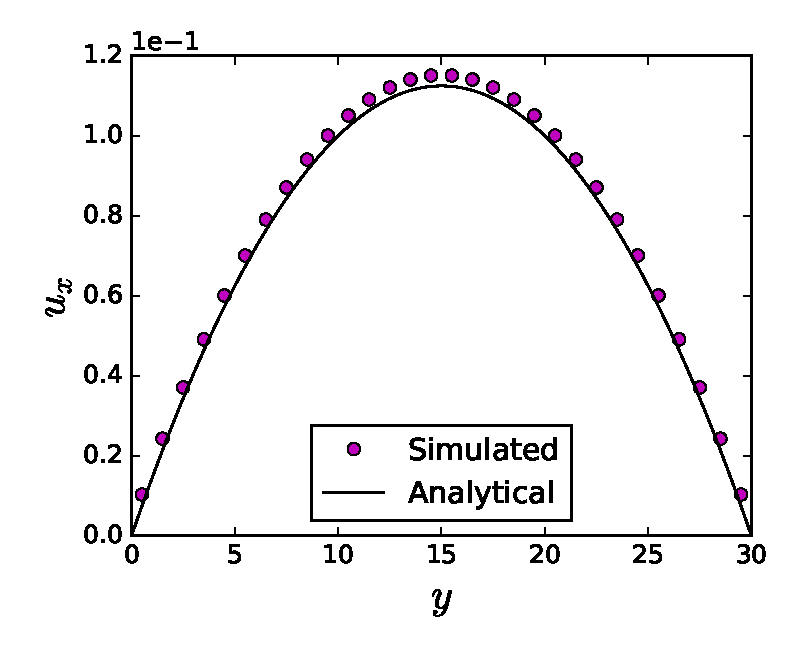
\includegraphics[width=\linewidth]{velocity_30}
	\label{fig:velocity_30}
\end{subfigure}\hfill
\begin{subfigure}{0.5\linewidth}
	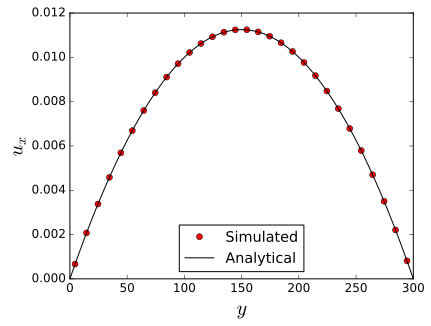
\includegraphics[width=\linewidth]{velocity_300}
	\label{fig:velocity_300}
\end{subfigure}
\medskip

\begin{subfigure}{0.5\linewidth}
	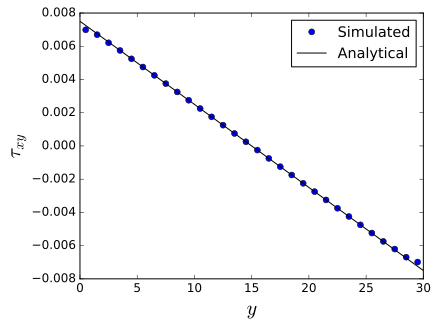
\includegraphics[width=\linewidth]{stressxy_30}
	\label{fig:stressxy_30}
\end{subfigure}\hfill
\begin{subfigure}{0.5\linewidth}
	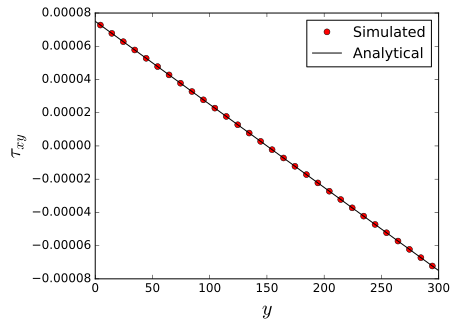
\includegraphics[width=\linewidth]{stressxy_300}
	\label{fig:stressxy_300}
\end{subfigure}
\caption{The $u_x$ component of velocity, and the $ \tau_{xy}$ components of extra stress with respect to $y$ position compared with their analytical solutions with $\eta_p = \eta_s = 0.5$, Re $= 6.75$, and Wi $= 1.125$ for $L_y = 30$ (left) and $L_y = 300$ (right).}
\label{fig:box_size_poiseuille}
\end{figure}

\begin{figure}
\begin{subfigure}{0.5\linewidth}
	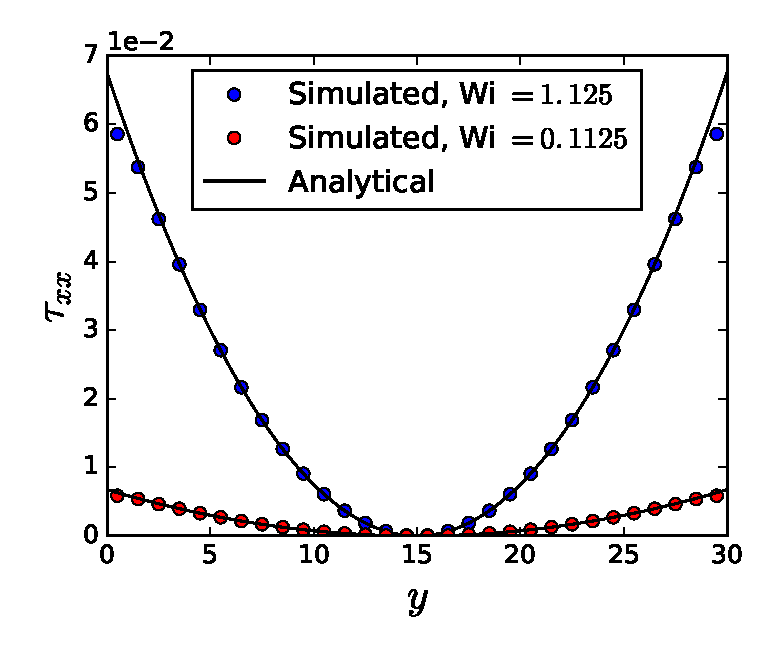
\includegraphics[width=\linewidth]{stressxx}
	\label{fig:stressxx}
\end{subfigure}\hfill
\begin{subfigure}{0.5\linewidth}
	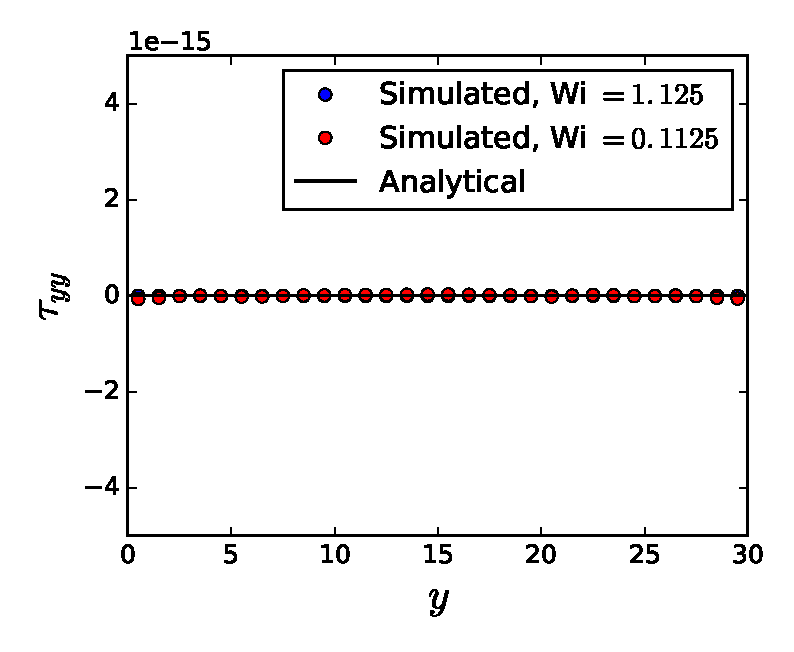
\includegraphics[width=\linewidth]{stressyy}
	\label{fig:stressyy}
\end{subfigure}
\caption{The the $ \tau_{xx}$ and $\tau_{yy}$ components of extra stress with respect to $y$ position compared with their analytical solutions with $\eta_p = \eta_s = 0.5$, Re $= 6.75$, and $L_y = 30$ for Wi $= 1.125$ and Wi $=0.1125$.}
\label{fig:diagonal_stress_poiseuille}
\end{figure}

\begin{figure}[htbp]
	\centering
	\begin{subfigure}{0.5\linewidth}
	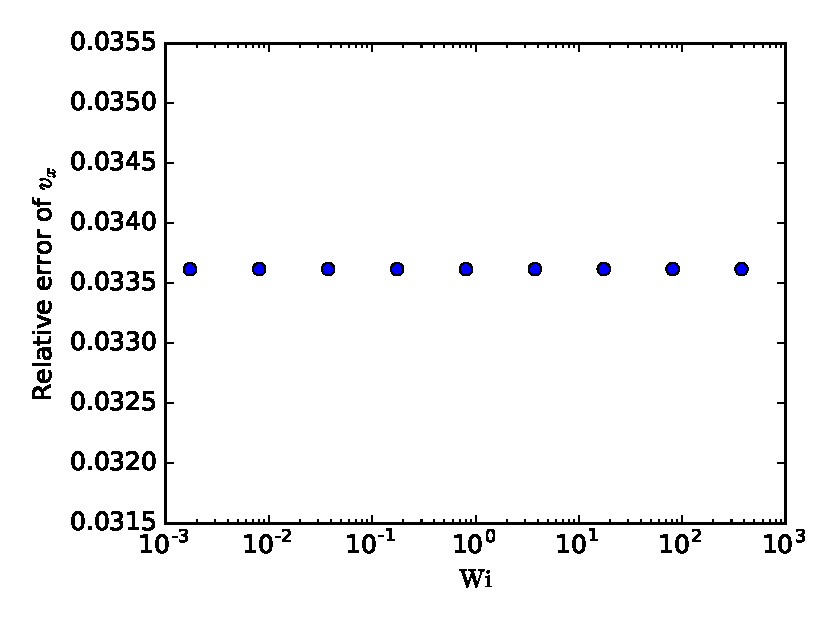
\includegraphics[width=\linewidth]{pois_vel_l2}
	\label{fig:stressxx_roll}
\end{subfigure}\medskip
\begin{subfigure}{0.5\linewidth}
	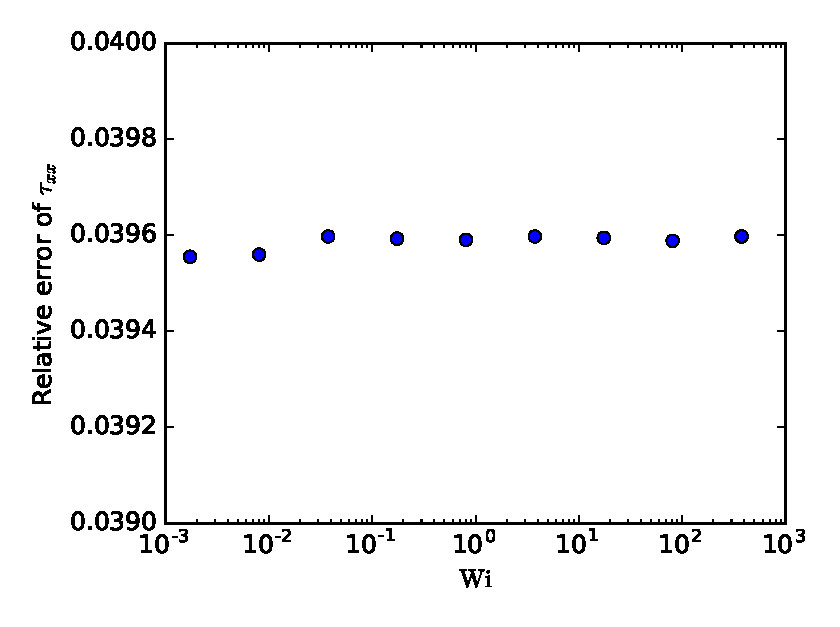
\includegraphics[width=\linewidth]{pois_xx_l2}
	\label{fig:stressxy_roll}
\end{subfigure}\hfill
\begin{subfigure}{0.5\linewidth}
	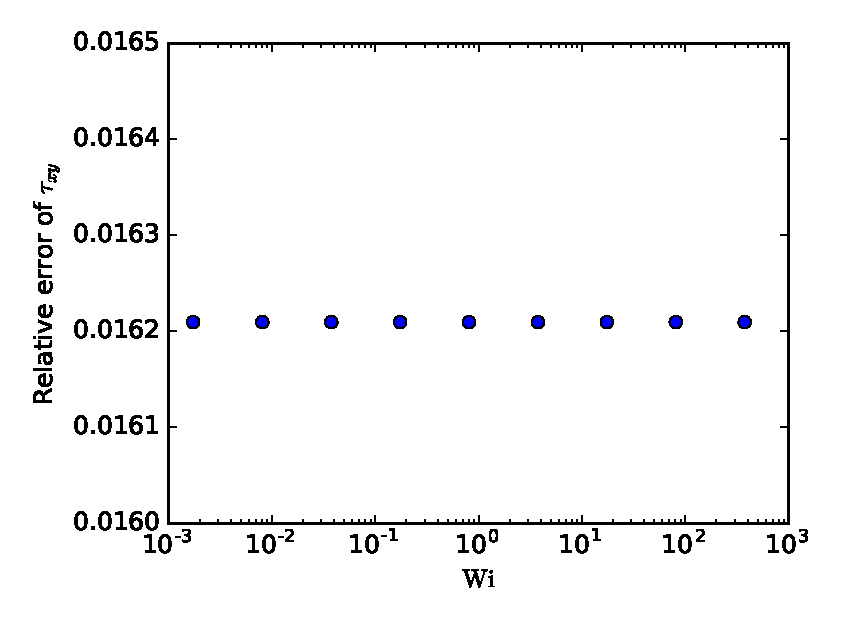
\includegraphics[width=\linewidth]{pois_xy_l2}
	\label{fig:stressyy_roll}
\end{subfigure}
\caption{$L_2$-norm error of $v_x$, $\tau_{xx}$, and $\tau_{xy}$ in Poiseuille flow for a wide range of Weissenberg numbers. Simualtions were performed with $L = 30$, $\eta_s = \eta_p = 0.5$ and $\mathrm{Re} = 0.0675$}
\label{fig:pois_error}
\end{figure}



\section{Four Roll Mill}
This benchmark simulates the effect of four cylinders rotating such that an elongational flow is created at the center point. We again approach this problem in two dimensions and use a body force to impose the effect of the mills. We use periodic boundary conditions in all directions so that we can focus on the bulk fluid. Fig.~\ref{fig:four_roll_sketch} shows a sketch of the system and forces along with the $\tau_{xy}$ component of extra stress in the flow. The imposed force density is given by
\begin{equation}\label{eq:four_mill_force}
\bm{f} = \frac{8\pi^2  \eta_s U_{\mathrm{max}}}{L^2}\lp\sin\lp\frac{2\pi}{L} x\rp\cos\lp\frac{2\pi}{L} y\rp, -\cos\lp\frac{2\pi}{L} x\rp\sin\lp\frac{2\pi}{L} y\rp\rp,
\end{equation}
where $L$ is the size of one dimension of the box and $U_\mathrm{max}$ is a parameter defining the magnitude of the same flow for a Newtonian fluid. It ensures that applying this force to a Newtonian fluid would result in the following flow profile:
\begin{equation}
\bm{u} = U_\mathrm{max}\lp-
\sin\lp\frac{2\pi}{L} x\rp\cos\lp\frac{2\pi}{L} y\rp, \cos\lp\frac{2\pi}{L} x\rp\sin\lp\frac{2\pi}{L} y\rp\rp.
\end{equation}
Additional viscosity due to the polymers will result in a lowered maximum velocity.

\begin{figure}[t]
	\centering
	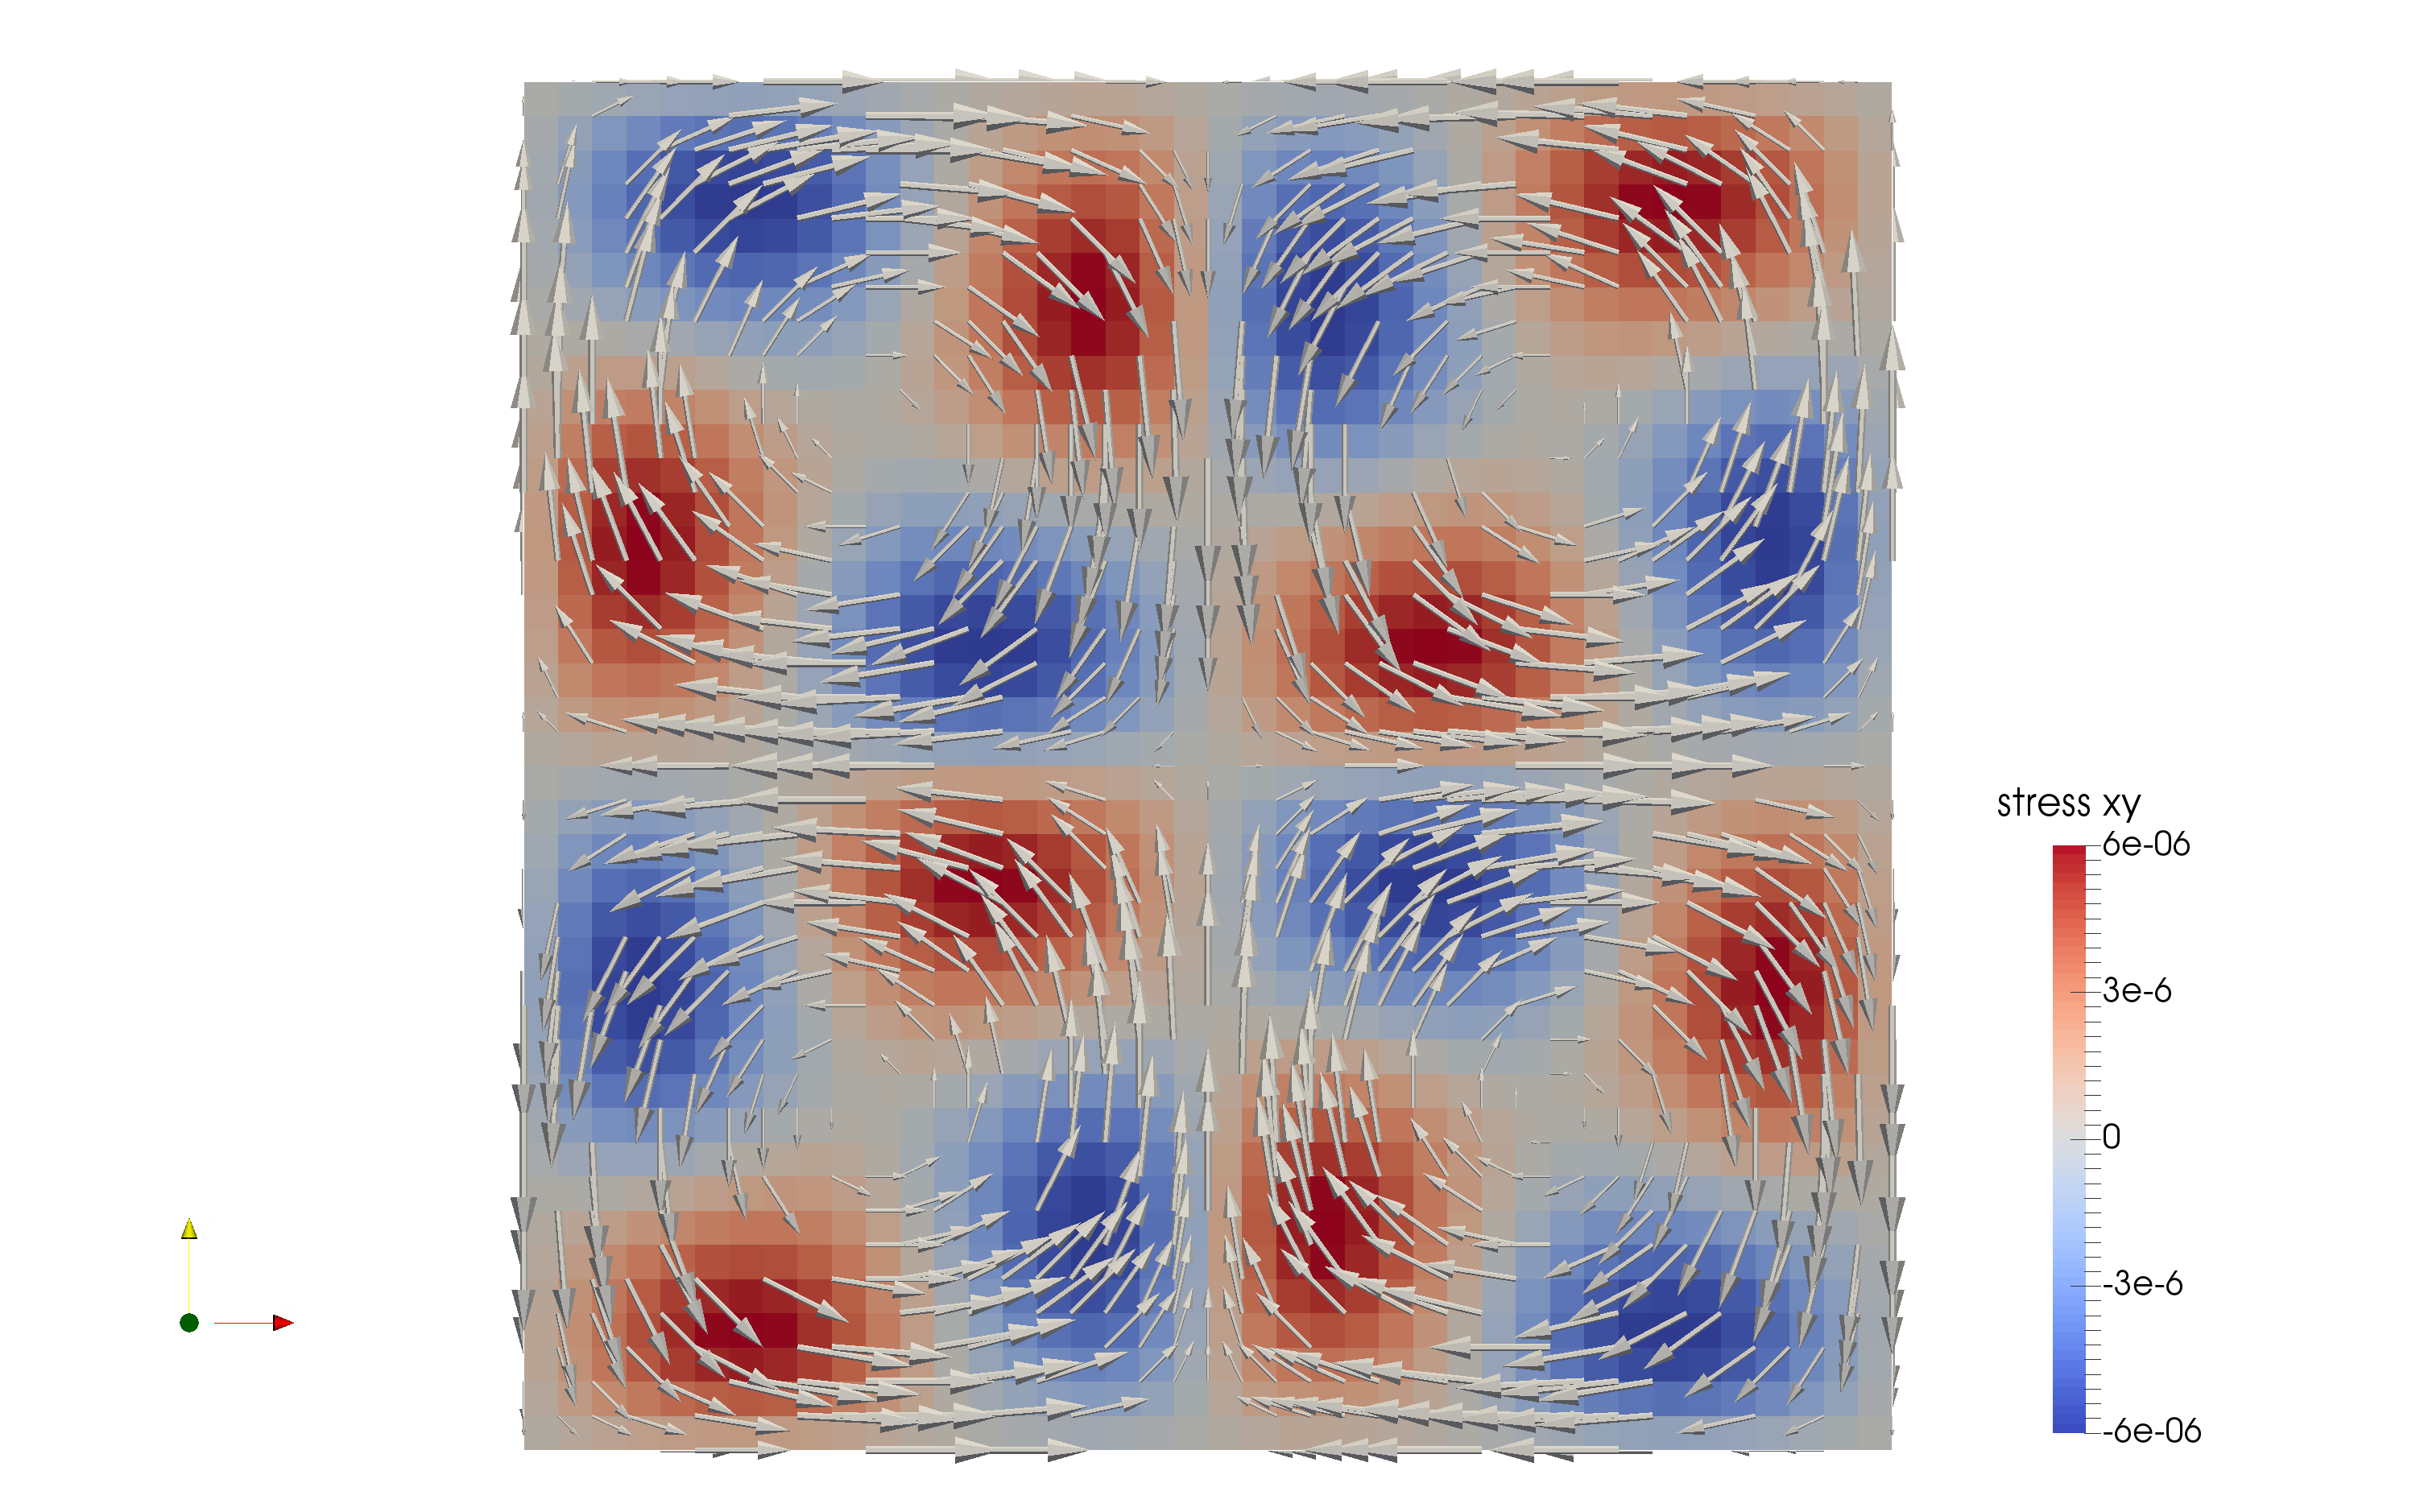
\includegraphics[width=\linewidth]{four_roll_sketch}
	\caption{The four roll mill system. The effect of the mills is given by a body force shown by the arrows. Also shown is the $\tau_{xy}$ component of extra stress.}
	\label{fig:four_roll_sketch}
\end{figure}

\subsection{Local Solution}
Since the four roll mill gives rise to a simple extensional flow at the center point, we would like to find an analytic solution for extensional flow with which to compare. The flow field for extensional flow is given by
\begin{equation}
\bm{u} = \alpha(x, -y),
\end{equation}
where $\alpha$ is some constant extention rate. This leaves us with a velocity gradient written as
\begin{equation}
\nabla\bm{u} = \lp\nabla \bm{u\rp}^\intercal = 
\begin{pmatrix}
\alpha & 0 \\
0 & -\alpha
\end{pmatrix}.
\end{equation}
We can then seperate Eq.~\eqref{eq:full_oldroyd_b} and solve for each component individually. We can demonstrate this first for the $\tau_{xx}$ component of the stress tensor. The equation we get from Eq.~\eqref{eq:full_oldroyd_b} becomes
\begin{equation}
\pardev{\txx}{t} + \alpha x \pardev{\txx}{x} - \alpha y \pardev{\txx}{y} + \lp \frac{1}{\lambda_p} - 2\alpha \rp \txx - \frac{2\eta_p \alpha}{\lambda_p} = 0.
\end{equation}
Multiplying by the reciprocal of the final term leaves us with
\begin{equation}
\frac{\gamma}{\alpha} \pardev{\txx}{t} + \gamma x \pardev{\txx}{x} - \gamma y \pardev{\txx}{y} +\lp \frac{\gamma}{\lambda_p} - 2\gamma\rp \txx =1,
\end{equation}
where we have defined
\begin{equation}
\gamma \defeq \frac{\lambda_p}{2 \eta_p}.
\end{equation}
Since we are interested in the steady state behavior, we may rescale the time by $\gamma/\alpha$ and 
rewrite the term in parenthesis leaving us with
\begin{equation}
\pardev{\txx}{t} + \gamma x \pardev{\txx}{x} - \gamma y \pardev{\txx}{y} + \beta \txx = 1,
\end{equation}
where
\begin{equation}
\beta \defeq \frac{\gamma}{\lambda_p} - 2\gamma.
\end{equation}
We can then find the general solution to this partial differential equation using the method of characteristics. \begin{figure}[tbp]
	\centering
\begin{subfigure}{0.5\linewidth}
	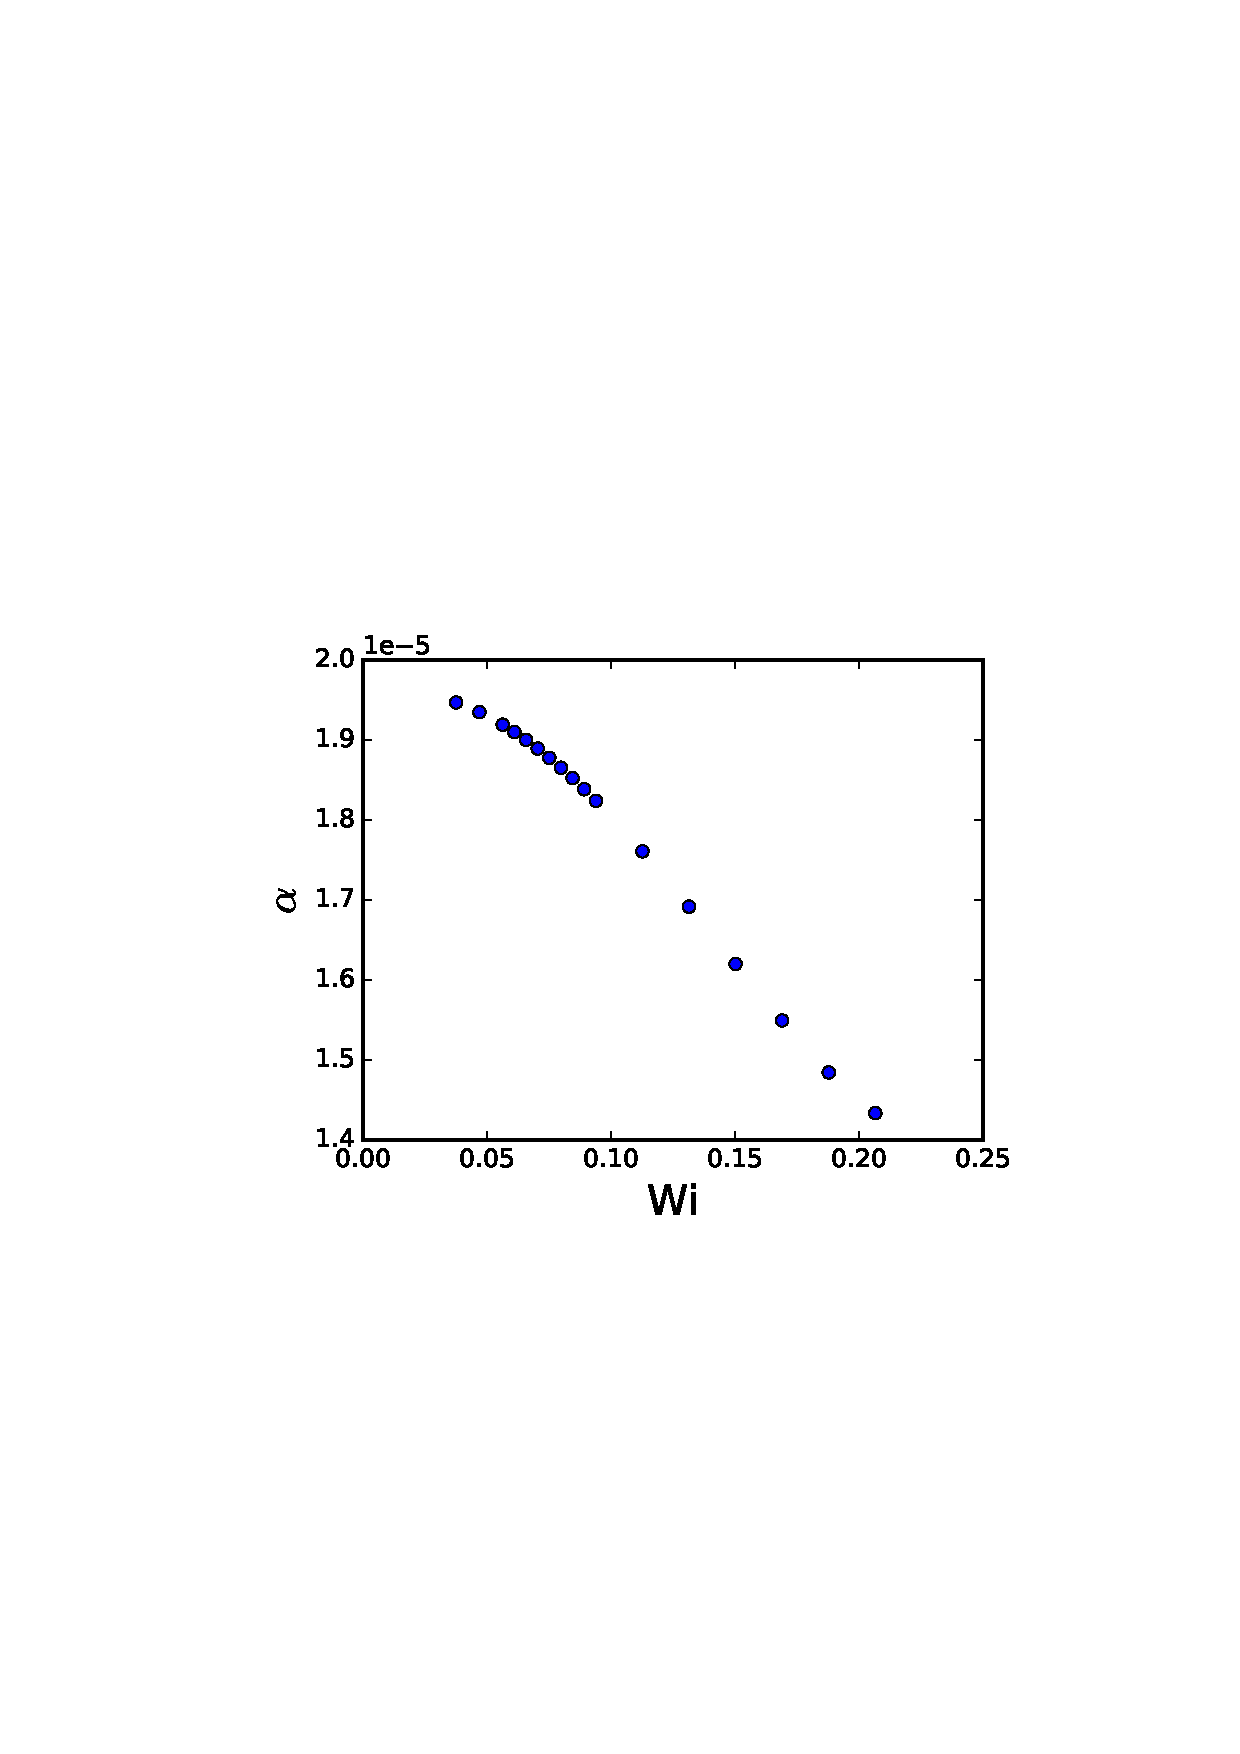
\includegraphics[width=\linewidth]{alpha_roll}
	\label{fig:alpha_roll}
\end{subfigure}\hfill
\begin{subfigure}{0.5\linewidth}
	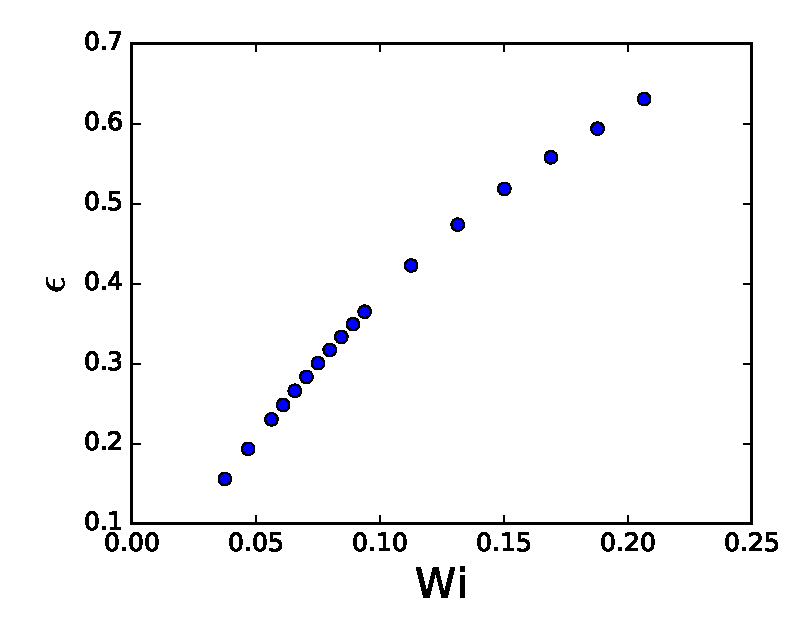
\includegraphics[width=\linewidth]{epsilon_roll}
	\label{fig:epsilon_roll}
\end{subfigure}
\caption{The elongation rate $\alpha$ (left) and effective Weissenberg number $\epsilon$ (right) as a function of Weissenberg number}
\label{fig:four_roll_parameters}
\end{figure}
The solution looks like
\begin{equation}\label{eq:tau_xx_general}
\txx(x,y,t) = \frac{1}{\beta} + e^{-\beta t}F_{xx}\lp xe^{-\gamma t}, ye^{\gamma t}\rp,
\end{equation}
where $F_{xx}$ is some arbitrary function. We consider solutions that depend little on $x$ and which are singular as $t \rightarrow \infty$. So choose $F_{xx}(a,b) \defeq f(b)$, where $f(b)\propto \lvert b\rvert^q$ as $b \rightarrow \infty$ for arbitrary $q$. Inserting into Eq.~\eqref{eq:tau_xx_general} gives
\begin{align}
\txx(x,y,t \rightarrow \infty) &= \frac{1}{\beta} + Ce^{-\beta t}\lvert ye^{\gamma t} \rvert^q \\
 &= \frac{1}{\beta} + Ce^{\lp\gamma q -\beta\rp t}\lvert y \rvert^q,
\end{align}
where $C$ is some constant. We require that the solution does not depend on $t$ at long times and so choose $q = \beta/\gamma$, i.e. 
\begin{align}
\txx(0,y) &= \frac{1}{\beta} + C \lvert y \rvert^\frac{\beta}{\gamma} \\
               &= \frac{2\eta_p\alpha}{1 - 2\epsilon} + C\lvert y\rvert^\frac{1-2\epsilon}{\epsilon},
\end{align}
where we have reinserted our original parameters and defined $\epsilon \defeq \alpha \lambda_p$ is the effective Weissenberg number. Similar analysis may be carried out to find the other components which are
\begin{equation}
\tau_{yy}(0,y) = -\frac{2\eta_p\alpha}{1 + 2\epsilon} + C\lvert y\rvert^\frac{1+2\epsilon}{\epsilon},
\end{equation}
\begin{equation}
\tau_{xy}(0,y) =0.
\end{equation}


\begin{figure}[tp]
	\centering
\begin{subfigure}{0.5\linewidth}
	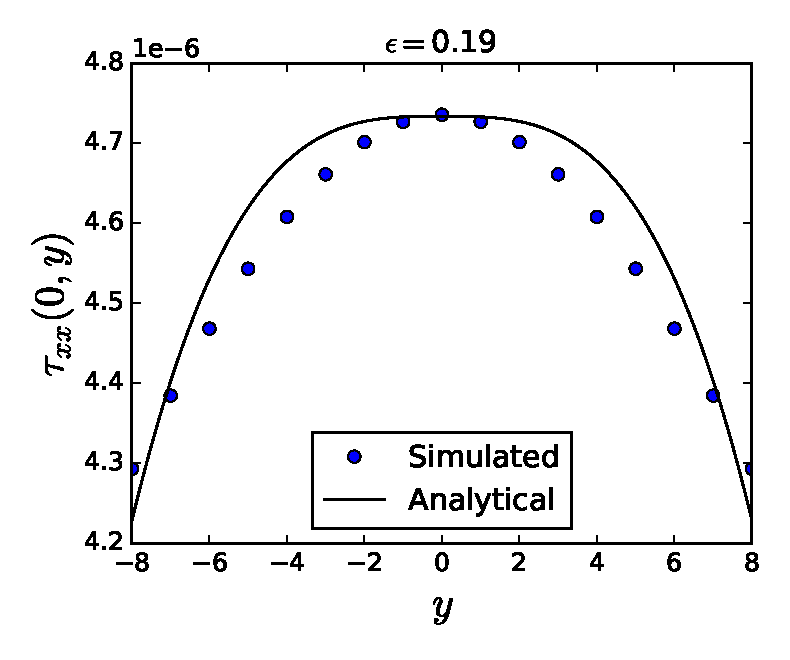
\includegraphics[width=\linewidth]{stressxx_10000_roll}
	\label{fig:stressxx_very_low}
\end{subfigure}\hfill
\begin{subfigure}{0.5\linewidth}
	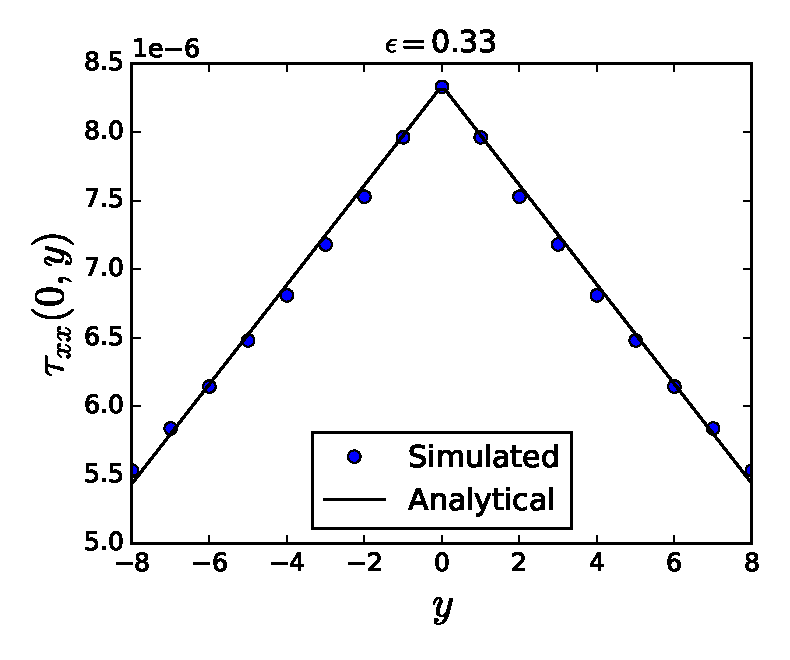
\includegraphics[width=\linewidth]{stressxx_18000_roll}
	\label{fig:stressxx_low}
\end{subfigure}
\medskip
\begin{subfigure}{0.5\linewidth}
	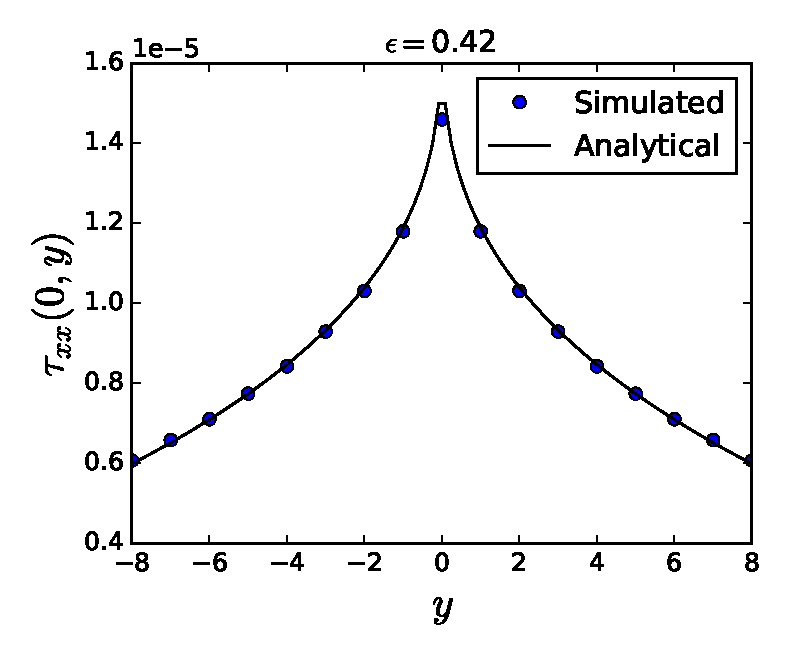
\includegraphics[width=\linewidth]{stressxx_24000_roll}
	\label{fig:stressxx_med}
\end{subfigure}\hfill
\begin{subfigure}{0.5\linewidth}
	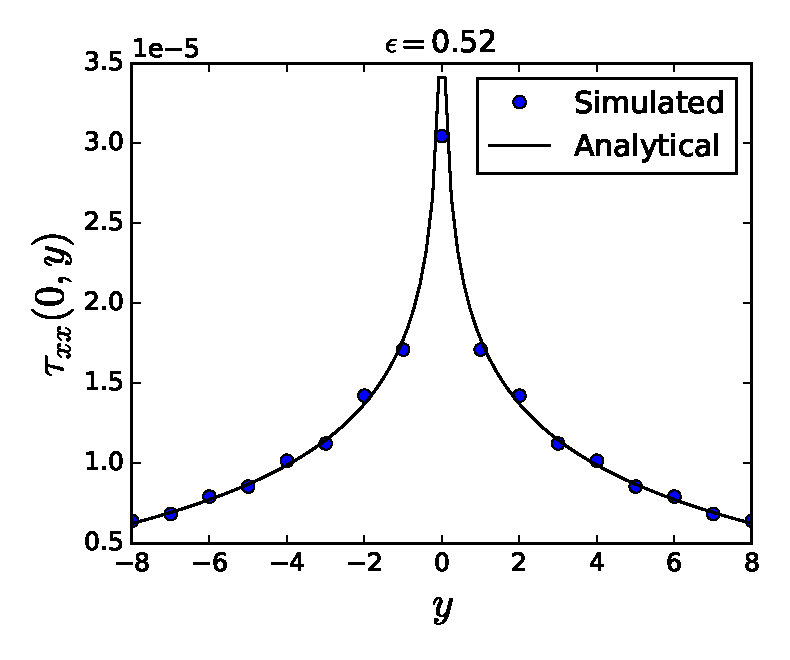
\includegraphics[width=\linewidth]{stressxx_32000_roll}
	\label{fig:stressxx_high}
\end{subfigure}
\caption{The $\tau_{xx}$ component of extra stress along the central vertical line in the Four Roll Mill for various effective Weissenberg numbers.}
\label{fig:stressxx_roll_group}
\end{figure}

\begin{figure}[htbp]
	\centering
\begin{subfigure}{0.5\linewidth}
	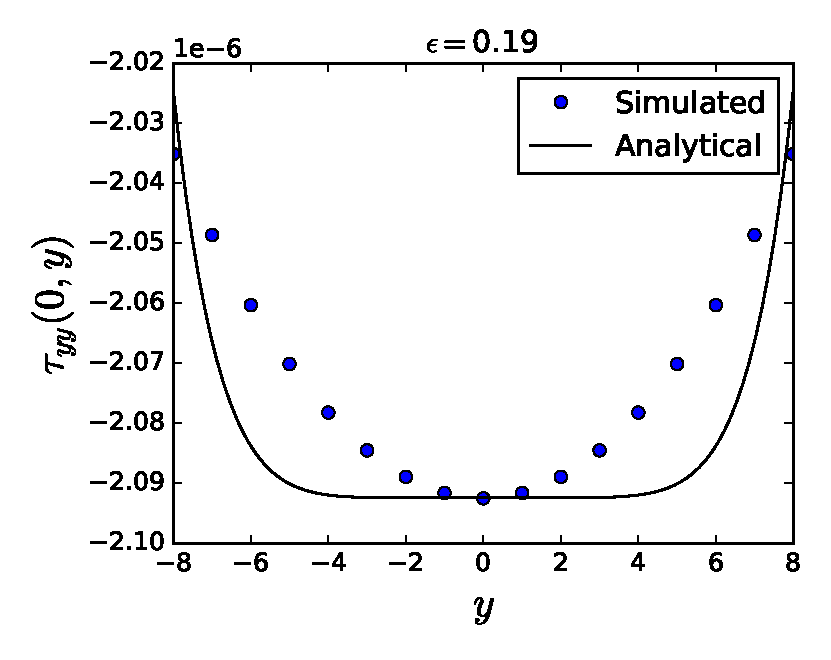
\includegraphics[width=\linewidth]{stressyy_10000_roll}
	\label{fig:stressyy_very_low}
\end{subfigure}\hfill
\begin{subfigure}{0.5\linewidth}
	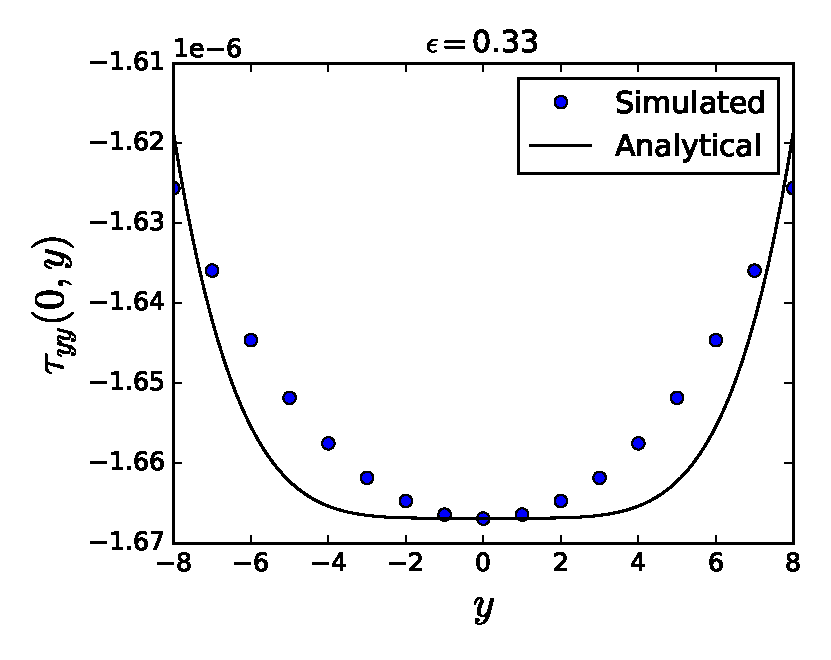
\includegraphics[width=\linewidth]{stressyy_18000_roll}
	\label{fig:stressyy_low}
\end{subfigure}
\medskip
\begin{subfigure}{0.5\linewidth}
	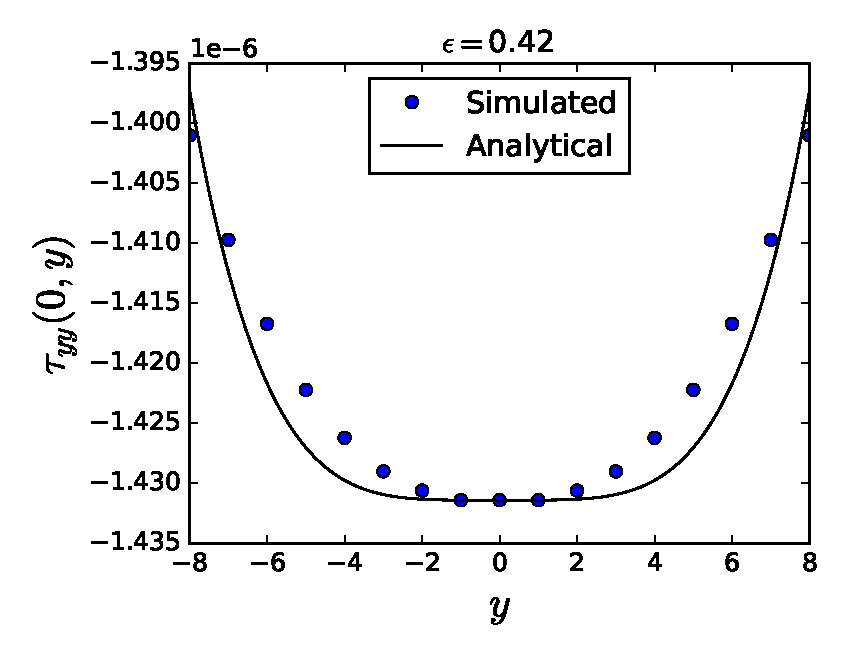
\includegraphics[width=\linewidth]{stressyy_24000_roll}
	\label{fig:stressyy_med}
\end{subfigure}\hfill
\begin{subfigure}{0.5\linewidth}
	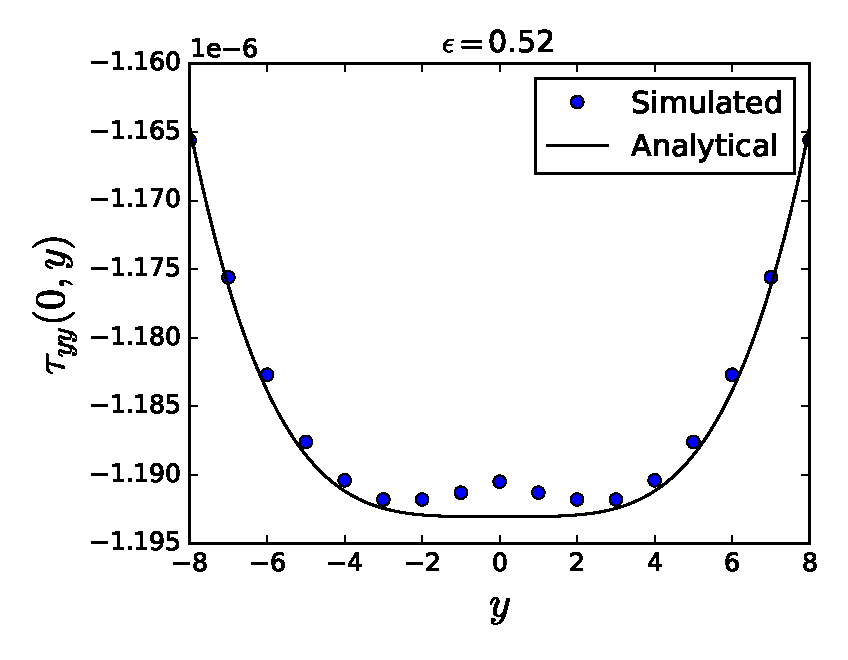
\includegraphics[width=\linewidth]{stressyy_32000_roll}
	\label{fig:stressyy_high}
\end{subfigure}
\caption{The $\tau_{yy}$ component of extra stress along the central vertical line in the Four Roll Mill for various effective Weissenberg numbers.}
\label{fig:stressyy_roll_group}
\end{figure}

\begin{figure}[htbp]
	\centering
	\begin{subfigure}{0.5\linewidth}
	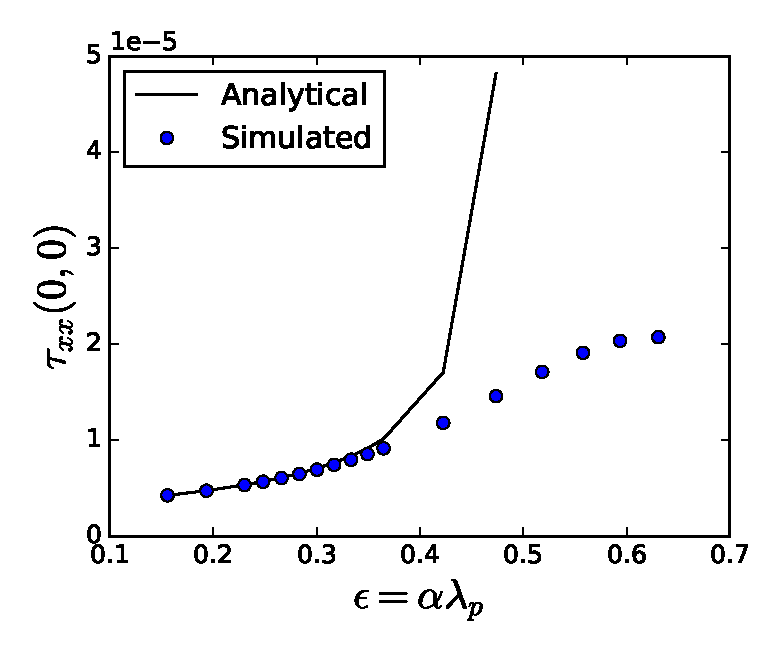
\includegraphics[width=\linewidth]{stressxx_roll}
	\label{fig:stressxx_roll}
\end{subfigure}\medskip
\begin{subfigure}{0.5\linewidth}
	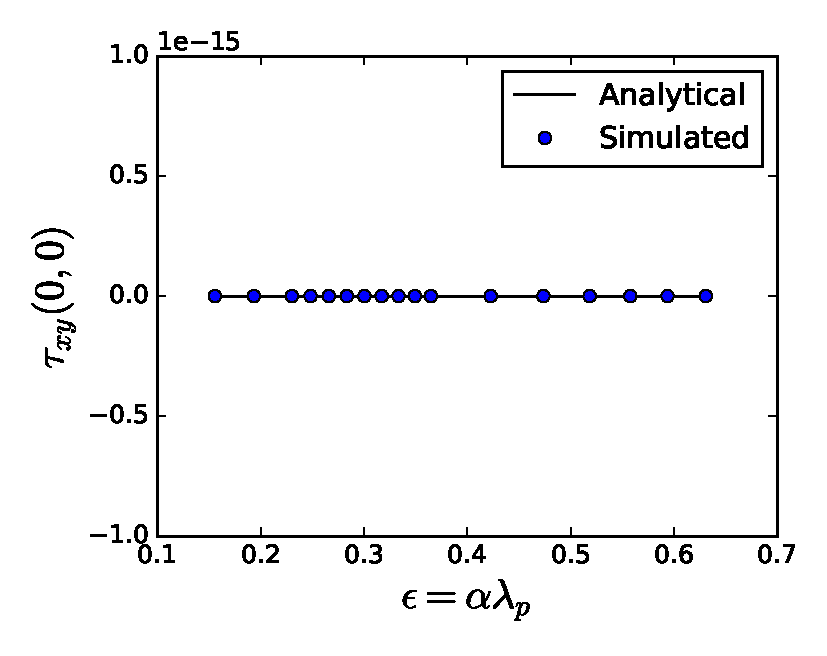
\includegraphics[width=\linewidth]{stressxy_roll}
	\label{fig:stressxy_roll}
\end{subfigure}\hfill
\begin{subfigure}{0.5\linewidth}
	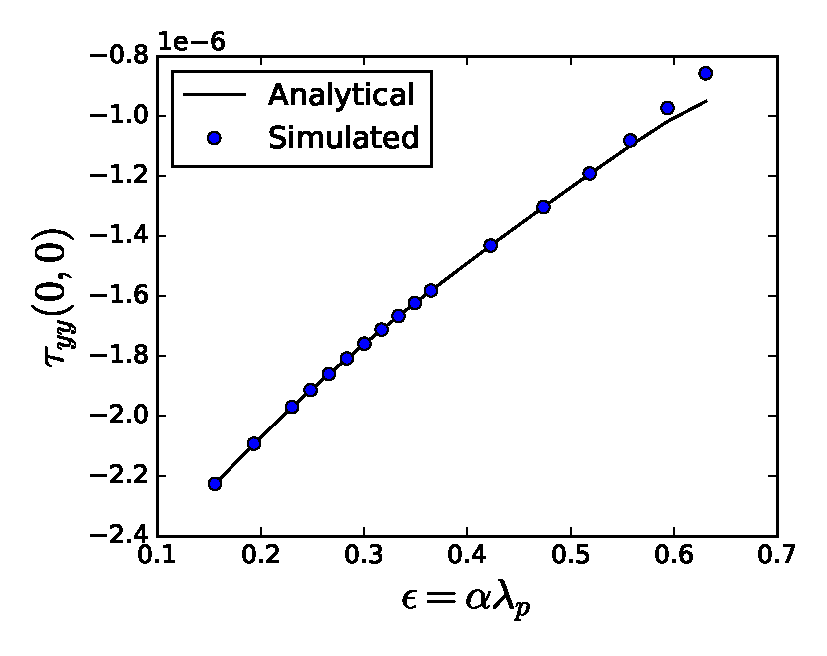
\includegraphics[width=\linewidth]{stressyy_roll}
	\label{fig:stressyy_roll}
\end{subfigure}
\caption{All three extra stress components as a function of effective Weissenberg number $\epsilon$ at the central point compared with the analytical value. Simulations carried out for varying polymer relaxation time.}
\label{fig:centerpoint_stress}
\end{figure}

\begin{figure}[htbp]
	\centering
	\begin{subfigure}{0.5\linewidth}
	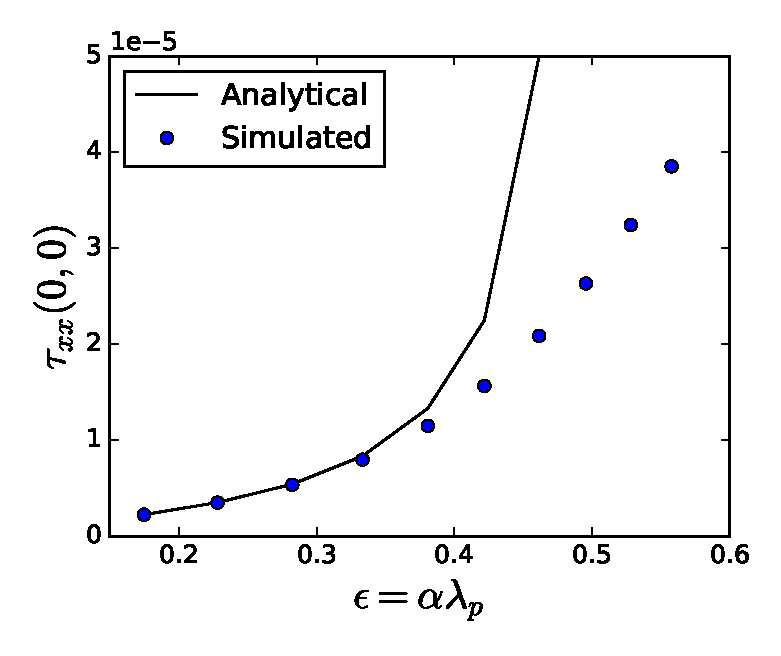
\includegraphics[width=\linewidth]{stressxx_alpha_roll}
	\label{fig:stressxx_alpha_roll}
\end{subfigure}\medskip
\begin{subfigure}{0.5\linewidth}
	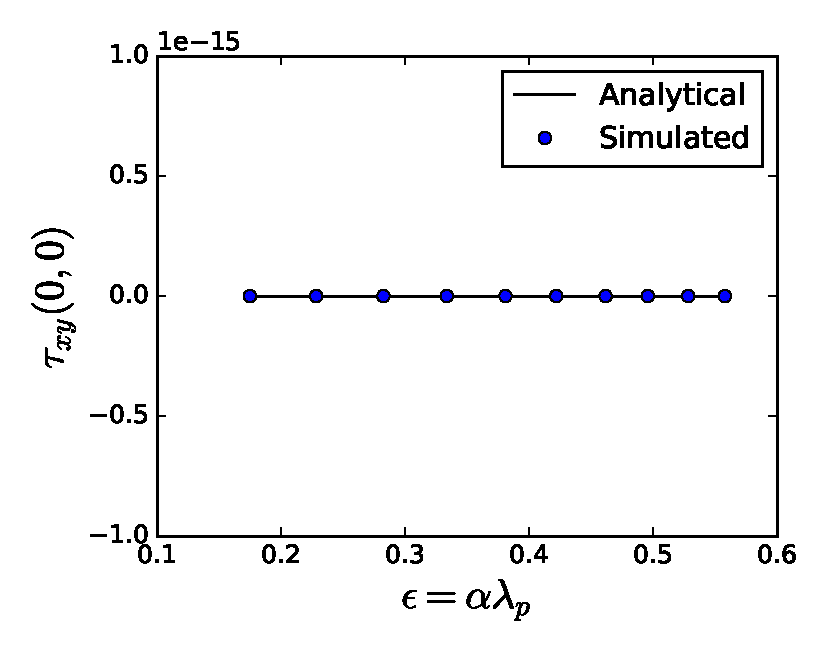
\includegraphics[width=\linewidth]{stressxy_alpha_roll}
	\label{fig:stressxy_alpha_roll}
\end{subfigure}\hfill
\begin{subfigure}{0.5\linewidth}
	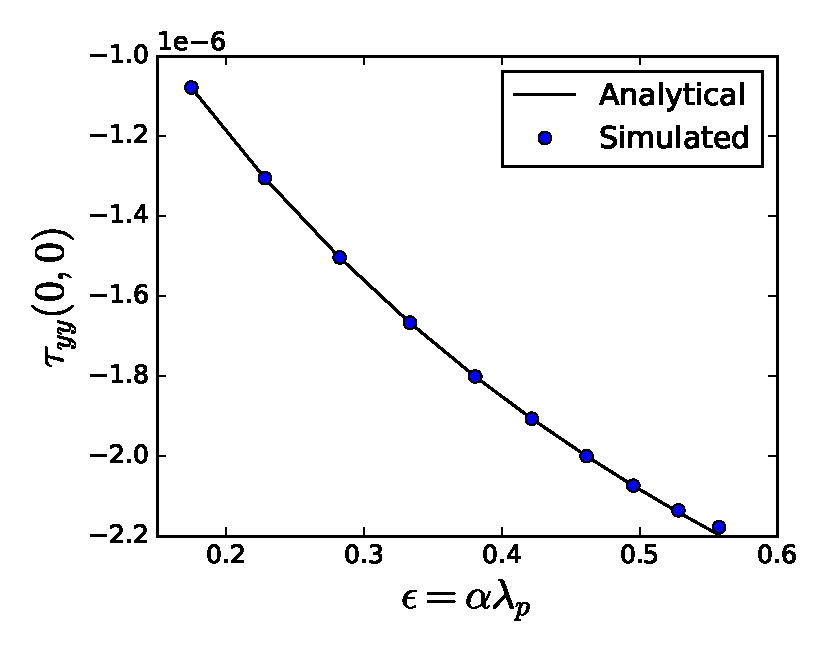
\includegraphics[width=\linewidth]{stressyy_alpha_roll}
	\label{fig:stressyy_alpha_roll}
\end{subfigure}
\caption{All three extra stress components as a function of effective Weissenberg number $\epsilon$ at the central point compared with the analytical value. Simulations carried out for varying force magnitude.}
\label{fig:centerpoint_stress_alpha}
\end{figure}

